\documentclass[a4paper,11pt,twocolumns]{article}
%\documentclass[dvips]{article}
\usepackage{graphicx}
\usepackage[spanish,activeacute]{babel}
\usepackage[margin=0.8in]{geometry}
\bibliographystyle{plain}
\usepackage{hyperref}
\usepackage{amssymb,amsmath}
\usepackage{draftwatermark}
\usepackage{graphicx}
\SetWatermarkFontSize{40pt}
\SetWatermarkScale{6}
\begin{document}

\twocolumn

\title{Midiendo la Performance de SPDY}
\author{Pablo Maximiliano Lulic}

\maketitle

\begin{abstract} 
Actualmente, la Web se sustenta con el est'andar \textsc{http}. Este protocolo tuvo su 'ultima versi'on en el a'no 1999. L'as p'aginas en ese entonces eran muy diferentes a las actuales, tanto en contenido como en recursos. Google desarroll'o un protocolo en el a'no 2009 llamado \textsc{spdy}, cuyo prop'osito es mejorar la performance en la recuperaci'on de los recursos de la web. A pesar de su gran aceptaci'on y de sentar las bases del pr'oximo \textsc{http 2.0}, hay ciertas cuestiones que todav'ia quedan por revisar. En este paper, se propone evaluar la performance de \textsc{spdy} desde dos enfoques diferentes, uno en embientes espec'ificos y otro en la web.
\end{abstract}

\section{Introducci'on}

El protocolo \textsc{http} tuvo su primera versi'on en mayo de 1996, culminando en 1999 con el est'andar actual que es el \textsc{http}  1.1 \cite{rfcHTTP} Es un protocolo sin estado, el servidor no mantiene informaci'on acerca de las diferentes peticiones que le llegan, lo que conlleva a que se necesite realizar una conexi'on nueva por cada recurso que se necesite de un sitio web.

\section{La Web en la Actualidad}

En comparaci'on con lo que era la web en la 'epoca en la que se implement'o el protocolo \textsc{http}, hubo un crecimiento amplio en el tama'no y en la cantidad de recursos de un sitio web. Para Noviembre de 2013 \cite{httpArchive}, el tama'no promedio de un sitio era de 1614kb, en contraste con Noviembre de 2010 que el tama'no promedio era de 702kb, el aumento fue casi del 50\%. El crecimiento se produce con velocidad \cite{averageWebPage} y hay otras cuestiones relacionadas al tiempo de carga de una p'agina, no solo el ancho de banda \cite{moreBand}, sino por ejemplo, el \textsc{rtt}\footnote{Tiempo que tarda un paquete de datos en ir desde el emisor al receptor y volver al emisor.}.

\section{SPDY}

\textsc{spdy}\cite{SPDYWhitepaper} es un protocolo de la capa de aplicaci'on \cite{illustratedTCPIP} que funciona sobre SSL \cite{rfcSSL}, permite la transmisi'on de Streams\footnote{???} sobre una conexi'on normal de \textsc{tcp}, que es el Protocolo de Control de Transmisi'on de la capa de Transporte \cite{illustratedTCPIP}). A continuaci'on se comentar'an las caracter'isticas del Protocolo (extra'idas de \cite{SPDYWhitepaper}):

\begin{enumerate}

\item Streams Multiplexados.

\item Priorizaci'on de Peticiones.

El Cliente puede tantos recursos como quiera del Servidor y asignarle prioridad a cada uno de ellos.

\item Compresi'on de los Headers \textsc{http} \cite{headersHTTP}.

Comprime los headers de petici'on y respuesta \textsc{http}.

\item Push

Permite al Servidor enviarle recursos al Cliente sin que este se lo pida.

\item Hint

Permite al Servidor ''sugerirle'' al Cliente que pida alg'un recurso espec'ifico.

\end{enumerate}

\section{Experimento 1}

\subsection{Preparaci'on}

Se utilizaron 3 computadoras de escritorio con la siguiente topolog'ia:

\vspace*{1\baselineskip}
\begin{math}
\frac{\textbf{CLIENTE}}{Debian GNU/Linux 6.0} \longleftrightarrow \frac{\textbf{PROXY}}{PicoBSD \cite{picoBSD}}  \longleftrightarrow \frac{\textbf{SERVIDOR}}{Lubuntu 13.04} 
\end{math}

\vspace*{1\baselineskip}

\begin{enumerate}
\item SERVIDOR

Se descargaron los sitios\footnote{Utilizando la opci'on ''Guardar como...'' de Google Chrome, que obteniene todos los recursos externos y los almacena en una carpeta.} y se configuraron los siguientes hosts virtuales en el Servidor:
\begin{enumerate}
\item www.amazon.com
\item www.bing.com
\item login.yahoo.com
\item www.world-flags.com \cite{flags}
\end{enumerate}
Cada sitio se brind'o utilizando Apache 2.2 \cite{apache} tanto en \textsc{http} como en \textsc{https}, para brindar \textsc{spdy}, se instal'o mod\_spdy \cite{modSPDY}.

\item PROXY

Utilizando la herramienta Dummynet \cite{dummynet} que viene instalada con la distribuci'on de PicoBSD, se utilizaron diferentes comandos \cite{ipfw} para filtrar el tr'afico en la red\footnote{Ancho de Banda y Retardo.} y simular diferentes entornos.

\item CLIENTE

Se utiliz'o Google Chrome 27 a trav'ez de chrome-har-capturer \cite{harCapt}. Dicha herramienta interact'ua con Google Chrome por su API de depuraci'on remota \cite{debuggingChrome}.

\end{enumerate} 

\subsection{Metodolog'ia}

Con la idea de comparar los m'etodos \textsc{http}, \textsc{https} y \textsc{spdy} en diferentes ambientes, se definieron los siguientes valores:

\begin{tabular}{ l c r }
	Ancho de Banda (BW)  \\ \hline
  	100 Kbps \\
	256 Kbps \\
	512 Kbps \\
	1024 Kbps \\
	2048 Kbps \\
	5120 Kbps \\
	10240 Kbps \\
\end{tabular}
\vspace*{1\baselineskip}
\begin{tabular}{ l c r }
	Retraso (RTT) \\ \hline
  	10 ms \\
	50 ms \\
	100 ms \\
	200 ms \\
	250 ms \\
	500 ms \\
	\\
\end{tabular}

Se combinaron todos los Anchos de Banda con todos los Retrasos para cada uno de los m'etodos por p'agina\footnote{Por ejemplo: 100Kbps de Ancho de Banda con 100ms de Retraso accediendo al host virtual de Amazon por \textsc{https} (https://www.amazon.com).}, se repiti'o el experimento 5 veces y se promediaron los resultados.

\subsection{Resultados}

SEGUIR ACA

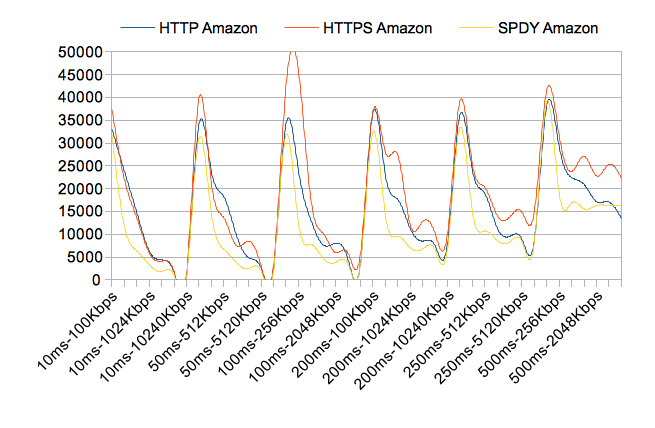
\includegraphics[scale=0.5]{res_amazon}

\section{Experimento 2}

\subsection{Preparaci'on}

\subsection{Metodolog'ia}

\subsection{Resultados}

\section{Conclusiones y Trabajos Relacionados}

\nocite{*}
\bibliography{bibliography}

\end{document}